\documentclass{article}
\usepackage[pdftex]{graphicx}

%Here are some good latex examples

\title{Dynamic Bayesian Networks\\An Introduction}

\author{Bill Davis}
\date{December 11, 2007}

\begin{document}
\maketitle

\begin{abstract}
Dynamic Bayesian Networks have been developed as a way to deal with probabilistic information that changes over time. Their complexity has lead to new techniques for both exact and approximate inference. This paper discusses these ideas as well as several case studies of practical application on Dynamic Bayesian Networks. 
\end{abstract}

%\pagebreak

\tableofcontents

\pagebreak

\section{Introduction}
Bayesian graphical models have become an increasingly important tool for managing uncertainty in complex systems. There has been extensive research in developing networks that encompass information in a wide array of subject matters, from medical diagnosis to financial planning.

Dynamic Bayesian networks were introduced as a means to codify standard techniques and methods that can be used to operate upon Bayesian networks under change. 

\section{Motivation}
Traditional Bayesian models have several limitations, one of the most prominent being that they are not designed to handle dynamic situations where the model may be changing as time progresses. \cite{mihajlovic2001}. As you might imagine, Dynamic Bayesian networks broadly defines systems whereby the standard Bayesian model is extended to support networks that are in states of change. Of course, even in the static models there are mechanisms to change the underlying model. Introducing evidence obviously changes the probability distribution over the network, and the introduction of virtual evidence alters the structure that the network employs. These mechanisms operate in a very simplistic fasion, and are not well adapted to systems which can change, in some cases dramatically, very frequently. Dynamic Bayesian Networks (DBN) are designed as a way to standardize a changing model and perhaps represent it in a less complicated way. This encourages the development of algorithms and techniques capable of dealing with them. DBNs can also allow models to change in ways that would be impossible to express simply with the introduction of evidence.

DBN is a term that seems to be somewhat overloaded, and is applied to both networks that are changing over time, "temporal" and also to networks which are changing as a result of "motive forces" \cite{sterritt00exploring}. A good example of the first is the described in \cite{oliverOffice}. Here a system was installed to monitor a person's office and make determinations about what was happening in that office over time. The system was trained to recognize several activities including phone conversations, working on the computer, presentations, etc. The driver here was data from sensors placed in the office that monitored sound, video and the keyboard and mouse. This data was obtained at regular intervals and drove decisions about the current state. 

As for the former \cite{group-model} consider using DBNs for group elevator control. Instead of time, the modal event is a new elevator request made by an arriving passenger. An indefinite amount of time may elapse between one elevator request and the next. The differences between these two ideas are usually conceptual instead of practical, and the algorithms designed for use with DBNs generally don't discriminate between the two concepts. The underlying models however, may be dependent upon the mode of update.  

\section {Definition}
\subsection{Markov Models}
Markov models were first developed to describe stochastic processes. They represent a way to introduce a random aspect to time-series data. Dynamic Bayesian networks can be seen as a generalization of Markov models. In the simplest case, a DBN can be viewed as a Markov chain. However there are extensions which can be used to express additional complexity that may be impossible to express using simpler Markov models.

\begin{figure}[h]
\begin{center}
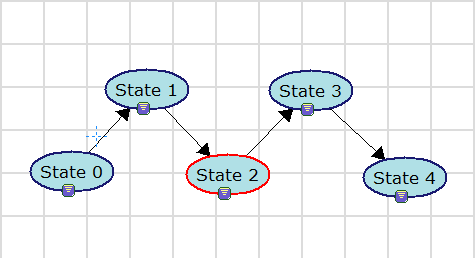
\includegraphics[height=40mm]{figures/simplemarkovmodel.png}
\caption{A Simple Markov Chain}
\label{fig:simplemarkovmodel}
\end{center}
\end{figure}

A Markov chain consists of both a finite number of states along with a set of probabilities $p_{ij}$ which is the probability of moving from state $i$ to state $j$ such that the probability of the next state is only dependent on the current state and not any state prior. That is for any sequence of outcomes $X_{1}, X_{2}, X_{3} ...$, $p(X_{n+1} | X_{n}, X_{n-1}, ..., X_{1}) = p(X_{n+1} | X_{n})$. This is called the Markov condition and it is the principal property of Markov models. 

\begin{figure}[h]
\begin{center}
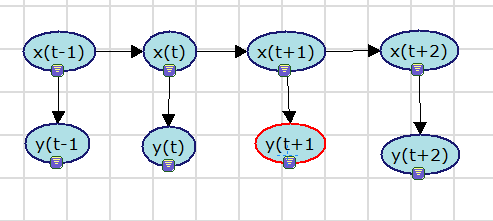
\includegraphics[height=40mm]{figures/hiddenmarkovmodel.png}
\caption{A Hidden Markov Model}
\label{fig:hiddenmarkovmodel}
\end{center}
\end{figure}

A hidden Markov model (HMM), is an extension of a Markov chain. The idea behind the HMM is that each observable state is dependent upon an unobserved or hidden variable. Here, each unobservered value $y_{n}$ is conditionally dependent only on $x_{n}$. Markov models are a well developed idea that has had applications in a number of fields. 

We can easily view these two ideas in the framework of dynamic Bayesian networks. For example, a Markov process is simply a dynamic Bayesian network consisting of $n$ Bayesian networks (BN) all stitched together, each static model containing a single random variable. The hidden Markov model is also a DBN consisting of $n$ BNs, but here each Bayesian network consists of 2 variables. The natural extension of these ideas is to pursue dynamic networks consisting of more arbitrary Bayesian networks all glued together. The practical problem when performing this extension is that complicated interdependencies can arise between time slices. 

For further reference regarding more complicated Markov models, including factorial hidden Markov Models and Tree Structured Hidden Markov models \cite {kuenzer-empirical} presents an empirical study analyzing the application of these models to syntactic user modeling. There is also an in-depth analysis of these models and more in \cite{murphy}. 

To further cement the relationship between DBNs and Markov Models, \cite{smyth96probabilistic} shows that the algorithms developed for use in Hidden Markov Models, specifically the forward-backward and Viterbi algorithms, are actually special case applications of the junction tree algorithm. 

\subsection{Dynamic Bayesian Networks}
DBNs are extensions to Markov models that add additional structure. A DBN is usually represented with two components. First there is a definition of a \emph{time slice}. This slice represents the state of the network at any given time period. The time slice is a traditionally defined Bayesian network. What makes the network dynamic is a definition of how the time slices influence each other over time. This is described by connecting nodes in one times slice to nodes in another. A first-order network contains links between adjacent time slices. A second order model connects a time slice to its two prior slices. Higher order networks can be constructed in a similar manner. This concept is shown in Figure~\ref{fig:timeslice} 

\begin{figure}[h]
\begin{center}
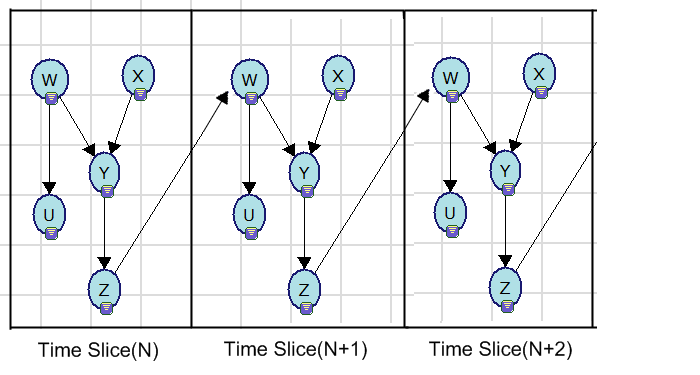
\includegraphics[height=40mm]{figures/timeslice.png}
\caption{3 Time Slices}
\label{fig:timeslice}
\end{center}
\end{figure}

\section{Inference in Dynamic Networks}
\subsection{Exact Inference}
The problem of exact inference in a static network can be suitably addressed using the join tree algorithm. The join tree can in fact also be applied to any defined DBN in a very straight forward way. Since any DBN network is composed of a series of interconnected time slices, we can theoretically create a static Bayesian network which is the composition of all of the time slices under consideration in the DBN. The problem, of course, when attempting computations over the unrolled static network, is that the complexity will almost certainly make exact inference using algorithms like the join tree intractable. This approach also throws out the symmetry which exists between all of the time slices.

In \cite{uk:dhugin} the details of one of the first approaches to dealing with the problem of inference in dynamic networks is described. The basic idea involves collecting multiple time slices into a time window. As the model evolves, new time slices are added to window and old ones are cut off. These processes are respectively called window expansion and window reduction. In this system there are three components to the model. A time window, which contains the time slices under consideration. A forecast window that contains slices we have not yet considered and a backwards window which contains slices which we have already considered, but have since discarded. These are show in Figure~\ref{fig:timewindow}. 

\begin{figure}[h]
\begin{center}
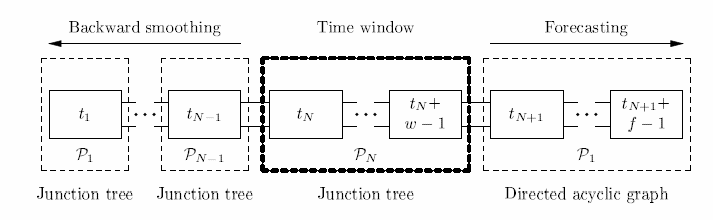
\includegraphics[height=40mm]{figures/timewindow.png}
\caption{The DBN expressed as a series of windows}
\label{fig:timewindow}
\end{center}
\end{figure}

Window expansion here encompasses several steps. First, moving new time slices into the forecast window. Then moving the oldest slices out of the forecast window into the current time window. The time window now needs to be triangulated and new cliques found. A new junction tree is then constructed of the current time window. Window reduction involves eliminating all the nodes which pertain to the time slices to be moved out of the current time window. Both acts require a triangulation, an expensive step, and can be coordinated to use the same elimination ordering. 

\subsection{Approximate Inference}
Since most dynamic belief networks are too extensively connected to use exact inference, several approximate inference techniques have been developed to deal with dynamic networks. Ultimately, the underlying problem is that, even though a given DBN may be able to be expressed in a structurally simplistic way, inference over that network still may be computationally intensive. Consider this example taken from \cite{boyentractable} in Figure~\ref{fig:complexity}.

\begin{figure}[h]
\begin{center}
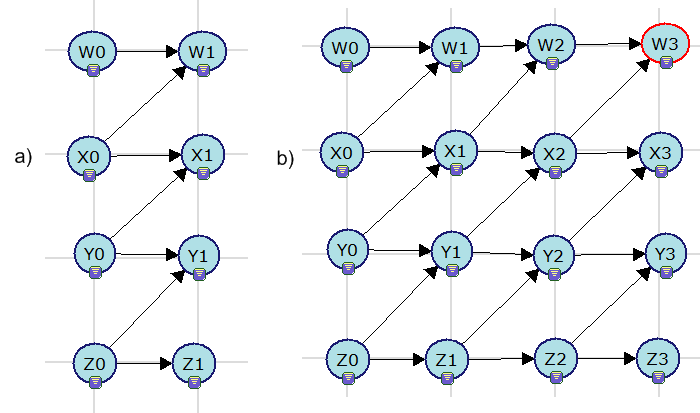
\includegraphics[height=50mm]{figures/complexity.png}
\caption{(a) shows the underlying structure of the network  (b) show how that networks looks extended over 4 time slices}
\label{fig:complexity}
\end{center}
\end{figure}

Initially all of the nodes in the network \{W, X, Y, Z\} start out conditionally independent. However, by the fourth time slice all of the nodes are now dependent upon one another. An exact inference computation over this network will grow computationally more difficult as the number of time slices under consideration grows. In order to perform approximate inference the normal stochastic simulation techniques, such as likelihood weighting and Gibbs sampling, can used for dynamic networks. One of the principal problems with this approach, however, is that their speed while sufficient for normal BNs, does not scale appropriately to deal with a large number of networks tied together. They operate at a performance disadvantage when compared to deterministic methods \cite{murphy92}. Therefore a significant area of research with regard to DBNs is ways to increase the performance of approximate techniques for inference. 

In \cite{boyentractable}, the researchers chose to deal with this complexity by generating an approximate belief state, one which is computationally tractable. They were able to find means to maintain an approximate belief state such that the resulting errors do not accumulate over time. They applied their approach to the DBN used in the BATmobile network which is discussed later. They achieved a 15 times speedup when performing approximate inference when compared to exact techniques, while maintaining relatively low error rates. 

\begin{figure}[h]
\begin{center}
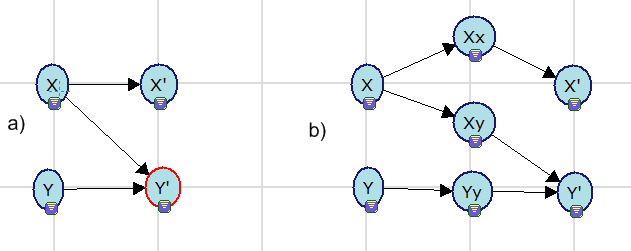
\includegraphics[height=30mm]{figures/bk.png}
\caption{(a) shows the original structure of the network  (b) shows how the original network is decomposed into independent components}
\label{fig:bk}
\end{center}
\end{figure}

The general process behind the Boyen-Koller algorithm is to project a given dynamic network onto another one with a marginally independent clusters of variables, while bounding the errors caused by the projection. In Figure~\ref{fig:bk}, the network in (a) is decomposed into the network in (b). Notice that the nodes added \{Xx, Xy, Yy\} d-separate the originals nodes \{X, Y\} from\{X', Y'\}. This process, however, maintains relatively loose error bounds.

An extension to the Boyen-Koller algorithm, Incremental Thin Junction Trees (ITJT), was introduced in \cite{hutter04incremental}. Their idea was to automatically detect set of independent clusters for use with the Boyen-Koller algorithm. It allows for the incremental building of approximate junction trees. This reduces the amount of computation when compared to other approximate junction algorithms, since ITIJ constructs approximate trees at each step as opposed to considering the DBN as a whole and creating an approximation off of it. 

\subsection{Learning}
One of the principal problems associated with Bayesian networks is producing prior conditional probabilities that can be used to initialize a network. Determining what these probabilities should be can be exceedingly difficult, especially in a complicated network which may have dozens of nodes. There has been a number of papers detailing methods whereby initial parameters of Bayesian networks can be learned from set of training data. These techniques can be applied with some success to dynamic networks \cite{ghahramani98learning}. Except in very simple cases, some approximation methods are needed in order to do this learning in a reasonable amount of time. Murphy also discusses in \cite{murphy} some "straightforward" extensions of static network techniques to perform both online and offline learning of dynamic network information. 

There have been some practical applications of these methods. In \cite{deviren01structural}, the author shows how DBNs can be used for speech recongnition. Here, even the structure of the DBN is able to be selected from a set of "realistic" structures along with the probability parameter information. 



\section{Examples}
There have been investigations into a number of practical applications of DBNs. Techniques have been developed for fields like robotic control, speech processing, and DNA analysis. Using DBNs to represent uncertainty works well in situations that can be modeled in ways that exhibit the Markov condition. Sometimes developing that kind of model is not straightforward, as for sentence analysis. In other scenarios it is very natural. For example, when performing robotic control, it is difficult to identify the position of a robot, given the sensor readings of the surroundings \cite{thrun98probabilistic}. At each time step however, the question is the same; given the various values obtained from the sensors coupled with the previous values and position of the robot, what is the current position of the robot? Normal application of Markov models to these problems is certainly possible, but by framing them as DBNs researchers can give the models added depth and perhaps more accurately represent the model underlying the situation. 

\subsection{BATMobile}
The BATmobile \cite{forbes95batmobile} was one of the first practical application of dynamic networks. The researchers used a 2-D traffic simulation to create realistic 3-D traffic data. This traffic data was then fed into the BATmobile, which was required to make intelligent decisions about acceleration, braking and lane-changing. Not only was the system designed to make these high-level decisions, it also had to implement them using low-level controls. Tight timing requirements when implementing a computer driven automobile, coupled with the complex manipulations of the network required by inference algorithms forced the BATmobile to introduce some techniques in order to reduce the amount of processing required per time step. The first was the use of temporally invariant networks, which is a network for which a node elimination operation produces a network which is identical to the original network. This kind of network is favorable to offline analysis which can find optimal elimination orderings that can be used during runtime of the program. 

\begin{figure}[here]
\begin{center}
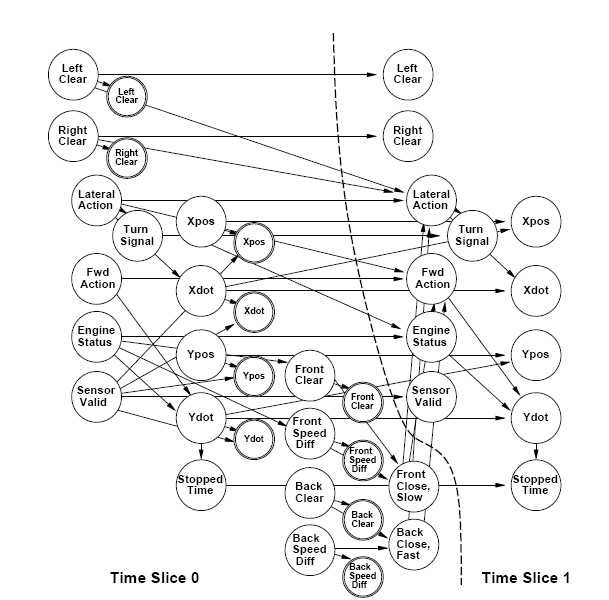
\includegraphics[height=100mm]{figures/batmobile.png}`
\caption{The BATmobile Vehicle Network}
\label{fig:batmobile}
\end{center}
\end{figure}

The network utilized by the BATmobile is show in Figure~\ref{fig:batmobile}.
The BATmobile made use of stochastic simulation for inference computations over this network. The researchers found that exact inference using a join tree was not only too expensive, but it was not necessary since approximate inference was sufficient. On the other hand, naive application of likelihood weighting also resulted in a traffic model which bore no resemblance to reality MUSTSAYMORE ABOUTHTISELSEWHERE. The conclusion made was that likelihood weighting simply ignores the input evidence introduced in the network, resulting in incorrect conclusions. The BATmobile introduced two methods to improve upon likelihood weighting; evidence reversal and survival of the fittest sampling. 

The BATmobile also experimented with three approaches to decision making, one of them being dynamic decision networks. These networks look much like dynamic belief networks, but at each time slice they contain a decision node. 

\subsection{Fall Prediction and Sensor Fusion} 
Fall prediction as applied to Bayesian networks encounters many of the same problems developed by the BATmobile. However, there is only one ultimate decision of interest to the network; whether or not a person has suffered a fall. In \cite{nicholson96case} the researchers developed a model for fall diagnosis. 
The dynamic network they generated is shown in Figure~\ref{fig:falldiagnosis}.

\begin{figure}[here]
\begin{center}
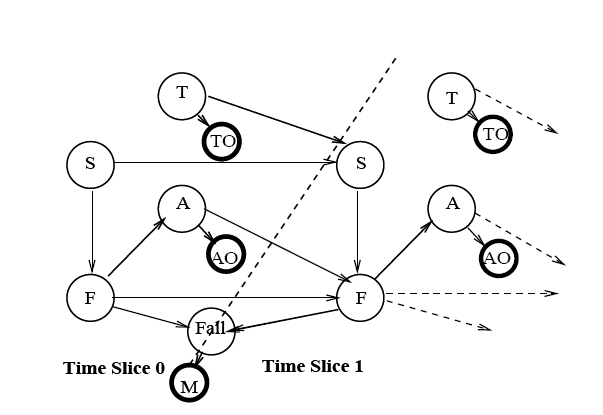
\includegraphics[height=40mm]{figures/falldiagnosis.png}
\caption{A DBN for fall diagnosis}
\label{fig:falldiagnosis}
\end{center}
\end{figure}

There variables of interest are defined as:
\begin{itemize}
\item 
Feet status (F). Possible values include both feet off the ground, both feet on the ground, left foot off the ground, and right foot off the ground. 
\item 
Time (T). The time between sensor observations.
\item 
Status (S). Whether the person is ok or stumbling. 
\item
Action (A). Has possible values left, right, none. 
\end{itemize}

Their model was successfully able to accurately diagnose a patient fall. Since the model they developed is nowhere near the complexity of the BATmobile, they did not enounter any performance issues. 

Since sensors were attached to both of the patients feet, the DBN had to be able to integrate the two sensor readings into a single concept of the world. This is a general problem encountered in many areas from radar analysis to weather prediction and is described as the concept of sensor fusion. Another example where a DBN was used for the process of sensor fusion is in \cite{btxhak}. There the authors showed how a DBN could be used to fuse GPS data with odometry data to select the most likely road on which a vehicle is traveling. There is an inherent probabalistic nature to fusing sensor data, each with their own error bounds. Using DBNs is natural way to resolve this disputing sensor information. In \cite{murphyspeech} the researchers were able to fuse visual features such as the contour of the lips and the position of the mouth with audio data to perform spech recongnition. The advantage to using DBNs in these sensor fusion scenarios is that they offer the oppertunity to backwards smooth the data, as well as perform future prediction. These actions are impossible using static networks since they only encompass knowledge of the current situation. 

\subsection{Grammatical Parsing and Applicability to Biological Models}
Parsing sentences for semantic information is not a straightforward task for a DBN, since the words in a sentence do not naturally exhibit the Markov property. We cannot, for example, simply extract the next word and feed it into the network because, in general, a semantic interpretation of a word may depend upon words that appear an arbitrary distance away. For this reason, we cannot simply generate a $n^{th}$ order DBN, because it would be unable to parse sentences information requiring n+1 understanding. An example will hopefully clarify this problem. 
\begin{enumerate}
\item
Bill wrote a paper.  
\item 
Bill thoughtfully wrote a paper.
\item 
Bill, slowly and deliberately, wrote a paper. 
\end{enumerate}

This example, in the spirit of \cite{savova2007} presents three different sentences. If we wish to build a system capable of determining that the general idea that Bill wrote something, we could use a normal Markov chain in the first example since those two words appear directly next two each other. But in the second sentence, we would need a $2^{nd}$ order model, since the word thoughtfully has now been placed between the subject and the verb. Of course in the third sentence we would need an even higher order model. In \cite{savova2007}, the researchers address this by deriving locally dependent variants for non-locally dependent sentences. 

In order to generate these locally dependent variants a DBN parser is generated from statistical information. The DBN parser is then fed a sentence and called recursively, at each layer attempting to determine the underlying dependency tree. The researchers claimed an 83\% success rate in determining the root dependency of a sentence. The parser they developed is show in Figure- ~\ref{fig:parsing}.

\begin{figure}[here]
\begin{center}
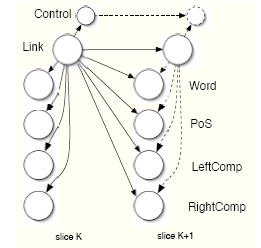
\includegraphics[height=45mm]{figures/parsing.png}
\caption{The parsing DBN used in \cite{savova2007}}
\label{fig:parsing}
\end{center}
\end{figure}

There is another issue with regard to DBN and sentence parsing, namely are Markov models in general, and DBNs specifically, relevant when it comes to the way humans interpret language. Savova and Peshkin claim that they are, since they were able to produce some understanding about sentence structure using a DBN. This information combined with the finding from \cite{rao2005} that networks of noisy integrate-and-fire neurons can perform approximate Bayesian inference for dynamic networks seems to indicate there is some possibility that DBNs do play a role in biological handling of language information. 
 
\section{Conclusion}
Dynamic Bayesian Networks were first introduced \cite{dk89}. Since then there has been a significant amount of work in fleshing out algorithms and techniques to simplify their application. This paper discusses some of that development and examined three specific applications of dynamic networks. 

%\nocite {*}
\bibliography{DBN}
\bibliographystyle{is-alpha}
\end{document}
